\section{Motivation and framework}

\begin{frame}{Limitations of GDP}
  \epigraph{"The welfare of a nation can scarcely be inferred from a measurement of national income"}{\textit{Simon Kuznets, 1934}}
  \pause
  GDP has become synonymous with welfare despite not capturing:
  \begin{enumerate}
    \item The value of the consumption of ecosystem services.
    \item The value of social factors.
  \end{enumerate}
  \vfill
  \note<1>{\textbf{MOTIVATION (1)}\\
    While Simon Kuznets' was in charge of developing the concept of GDP in the 1930s, he warned that \textbf{(...)}.\\
  }
  \note<2>{\textbf{MOTIVATION (2)}\\
  Nonetheless, GDP has largely become synonymous with welfare - which has led to criticism of its shortcomings in not capturing either (1) or (2).\\
  Therefore, there is a widespread search for alternative measures
  \begin{itemize}
    \item e.g. the European Commission has launched a \textbf{Beyond GDP initiative}, motivated as being 
    \textit{"about developing indicators that are as clear and appealing as GDP, but more inclusive of environmental and social aspects of progress. Economic indicators such as GDP were never designed to be comprehensive measures of prosperity and well-being."}
  \end{itemize}
}
\end{frame}


\begin{frame}{Why calculate a Green GDP?}
  Our estimation of a \textbf{Danish Green GDP} serves a triple purpose:
  \pause
  \begin{enumerate}
    \item Valuation allows summation and comparison of ecosystems.
    \pause
    \item Analyze whether economic development from 1990-2020 meets the criterion of "strong" sustainability?
    \pause
    \item Provide a measure that is directly comparable to the GDP.
  \end{enumerate}
  \vfill
  \note<1>{\textbf{TRIPLE PURPOSE}\\
    As a solution to the first shortcoming of GDP,\\
    we estimate a Danish Green GDP with a triple purpose:
  }
  \note<2>{\textbf{PURPOSE (1)}\\
    \begin{enumerate}
      \item Beyond just describing the water quality in biological terms, monetary \textbf{(...)} and indicates the WTP for improvements in a given ecosystem relative to consumption of conventional goods and costs of measures to improve the environment.
    \end{enumerate}
  }
  \note<3>{\textbf{PURPOSE (2)}\\
  \begin{enumerate}
    \item 
    \item Neither GDP nor the Green GDP should be interpreted as a measure for welfare, but the Green GDP is the attempt to \textbf{(...)} i.e. whether growth happened at the expense of the overall environment or allowed for a positive net growth in the environmental quality?
  \end{enumerate}
  }
  \note<4>{\textbf{PURPOSE (3)}\\
    \begin{enumerate}
      \item 
      \item 
      \item we do so using a measure that is directly comparable to the familiar concept of the GDP.
      \begin{itemize}
        \item Alternatively, one could simply use \textbf{Genuine Saving} but it's a is less known concept which is already included as a component of the Green GDP - which moreover includes the \textbf{current benefit} of the environmental quality.
      \end{itemize}
    \end{enumerate}
  }
\end{frame}


\begin{frame}{Research framework}
  Conventional Net National Income:
  \begin{align*}
    \textbf{NNI} = \text{GDP} &- \text{depreciation of manufactured capital} \\
    &+ \text{net foreign factor income}
  \end{align*}
  \pause
  \begin{tcolorbox}
    Green Net National Income:
    \begin{align*}
        \textbf{GNNI} = \text{NNI} &+ \text{\color{darkgreen}benefit of the environmental quality} \\
        &+ \text{\color{darkgreen}net growth in the environmental quality}
    \end{align*}
  \end{tcolorbox}
  \vfill
  \note<1>{\textbf{FRAMEWORK (1)}\\
    In the literature, the Green NNI is the preferred measure, while one can deduct the Green GDP from it.\\\bigskip
    The \textbf{NNI} can be written as \textbf{(...)}:\\\bigskip
    i.e. the NNI captures the annual output of Danish citizens both domestically and abroad before accounting for the environment.
  }
  \note<2>{\textbf{FRAMEWORK (2)}\\
    The \textbf{Green NNI} is defined as:\\\bigskip
    NNI\\
    +\textcolor{darkgreen}{current marginal benefit of the environmental quality} \\
    +\textcolor{darkgreen}{present value of net growth in environmental quality}
    \\\bigskip
    \textbf{[In more general terms - \textit{only if asked}]}\\
    +\textcolor{darkgreen}{value of consumption of environmental services} \\
    +\textcolor{darkgreen}{value of saving in environmental assets} \\\bigskip
    
  }
\end{frame}


\begin{frame}{Ecosystem services of waterbodies}
  \begin{table}\hspace{-.6cm}
    \scriptsize
      \begin{tabular}{l|c|c|c|} % the number of total columns and which have vertical lines between them (left-align or center text).
        \multicolumn{1}{c}{} & \multicolumn{3}{c}{Output of ecosystem services}\\ % "2" is the number of columns in the matrix that the 2nd player name spans over
        % \parbox[t]{1mm}{\multirow{3}{*}{\rotatebox[origin=r]{90}{Type}}} % "3" is the number of rows the 1st player name spans over (including the one with the column names)
        \multicolumn{1}{c}{} & \multicolumn{1}{c}{Provisioning services} & \multicolumn{1}{c}{Regulating services} & \multicolumn{1}{c}{Cultural services} \\\cline{2-4} % column names use the "\multicolumn" command to not draw vertical lines between them.
        Surface water & & Support of health & Biodiversity, recreation, aesthetic \\\cline{2-4} % a horizontal line is drawn after the line break using "\cline{x-y}" where x and y are the column numbers of the cells to be underlined.
        \pause
        Groundwater & Drinking water* & Support of health &  \\\cline{2-4}
      \end{tabular}
  \end{table}
  \pause
  Water quality can be damaged by:
  \begin{itemize}
    \item Physical modifications.
    \pause
    \item Nutrient overenrichment $\rightarrow$ algae growth $\rightarrow$ oxygen depletion.
  \end{itemize}
  \hspace{-.8cm}
  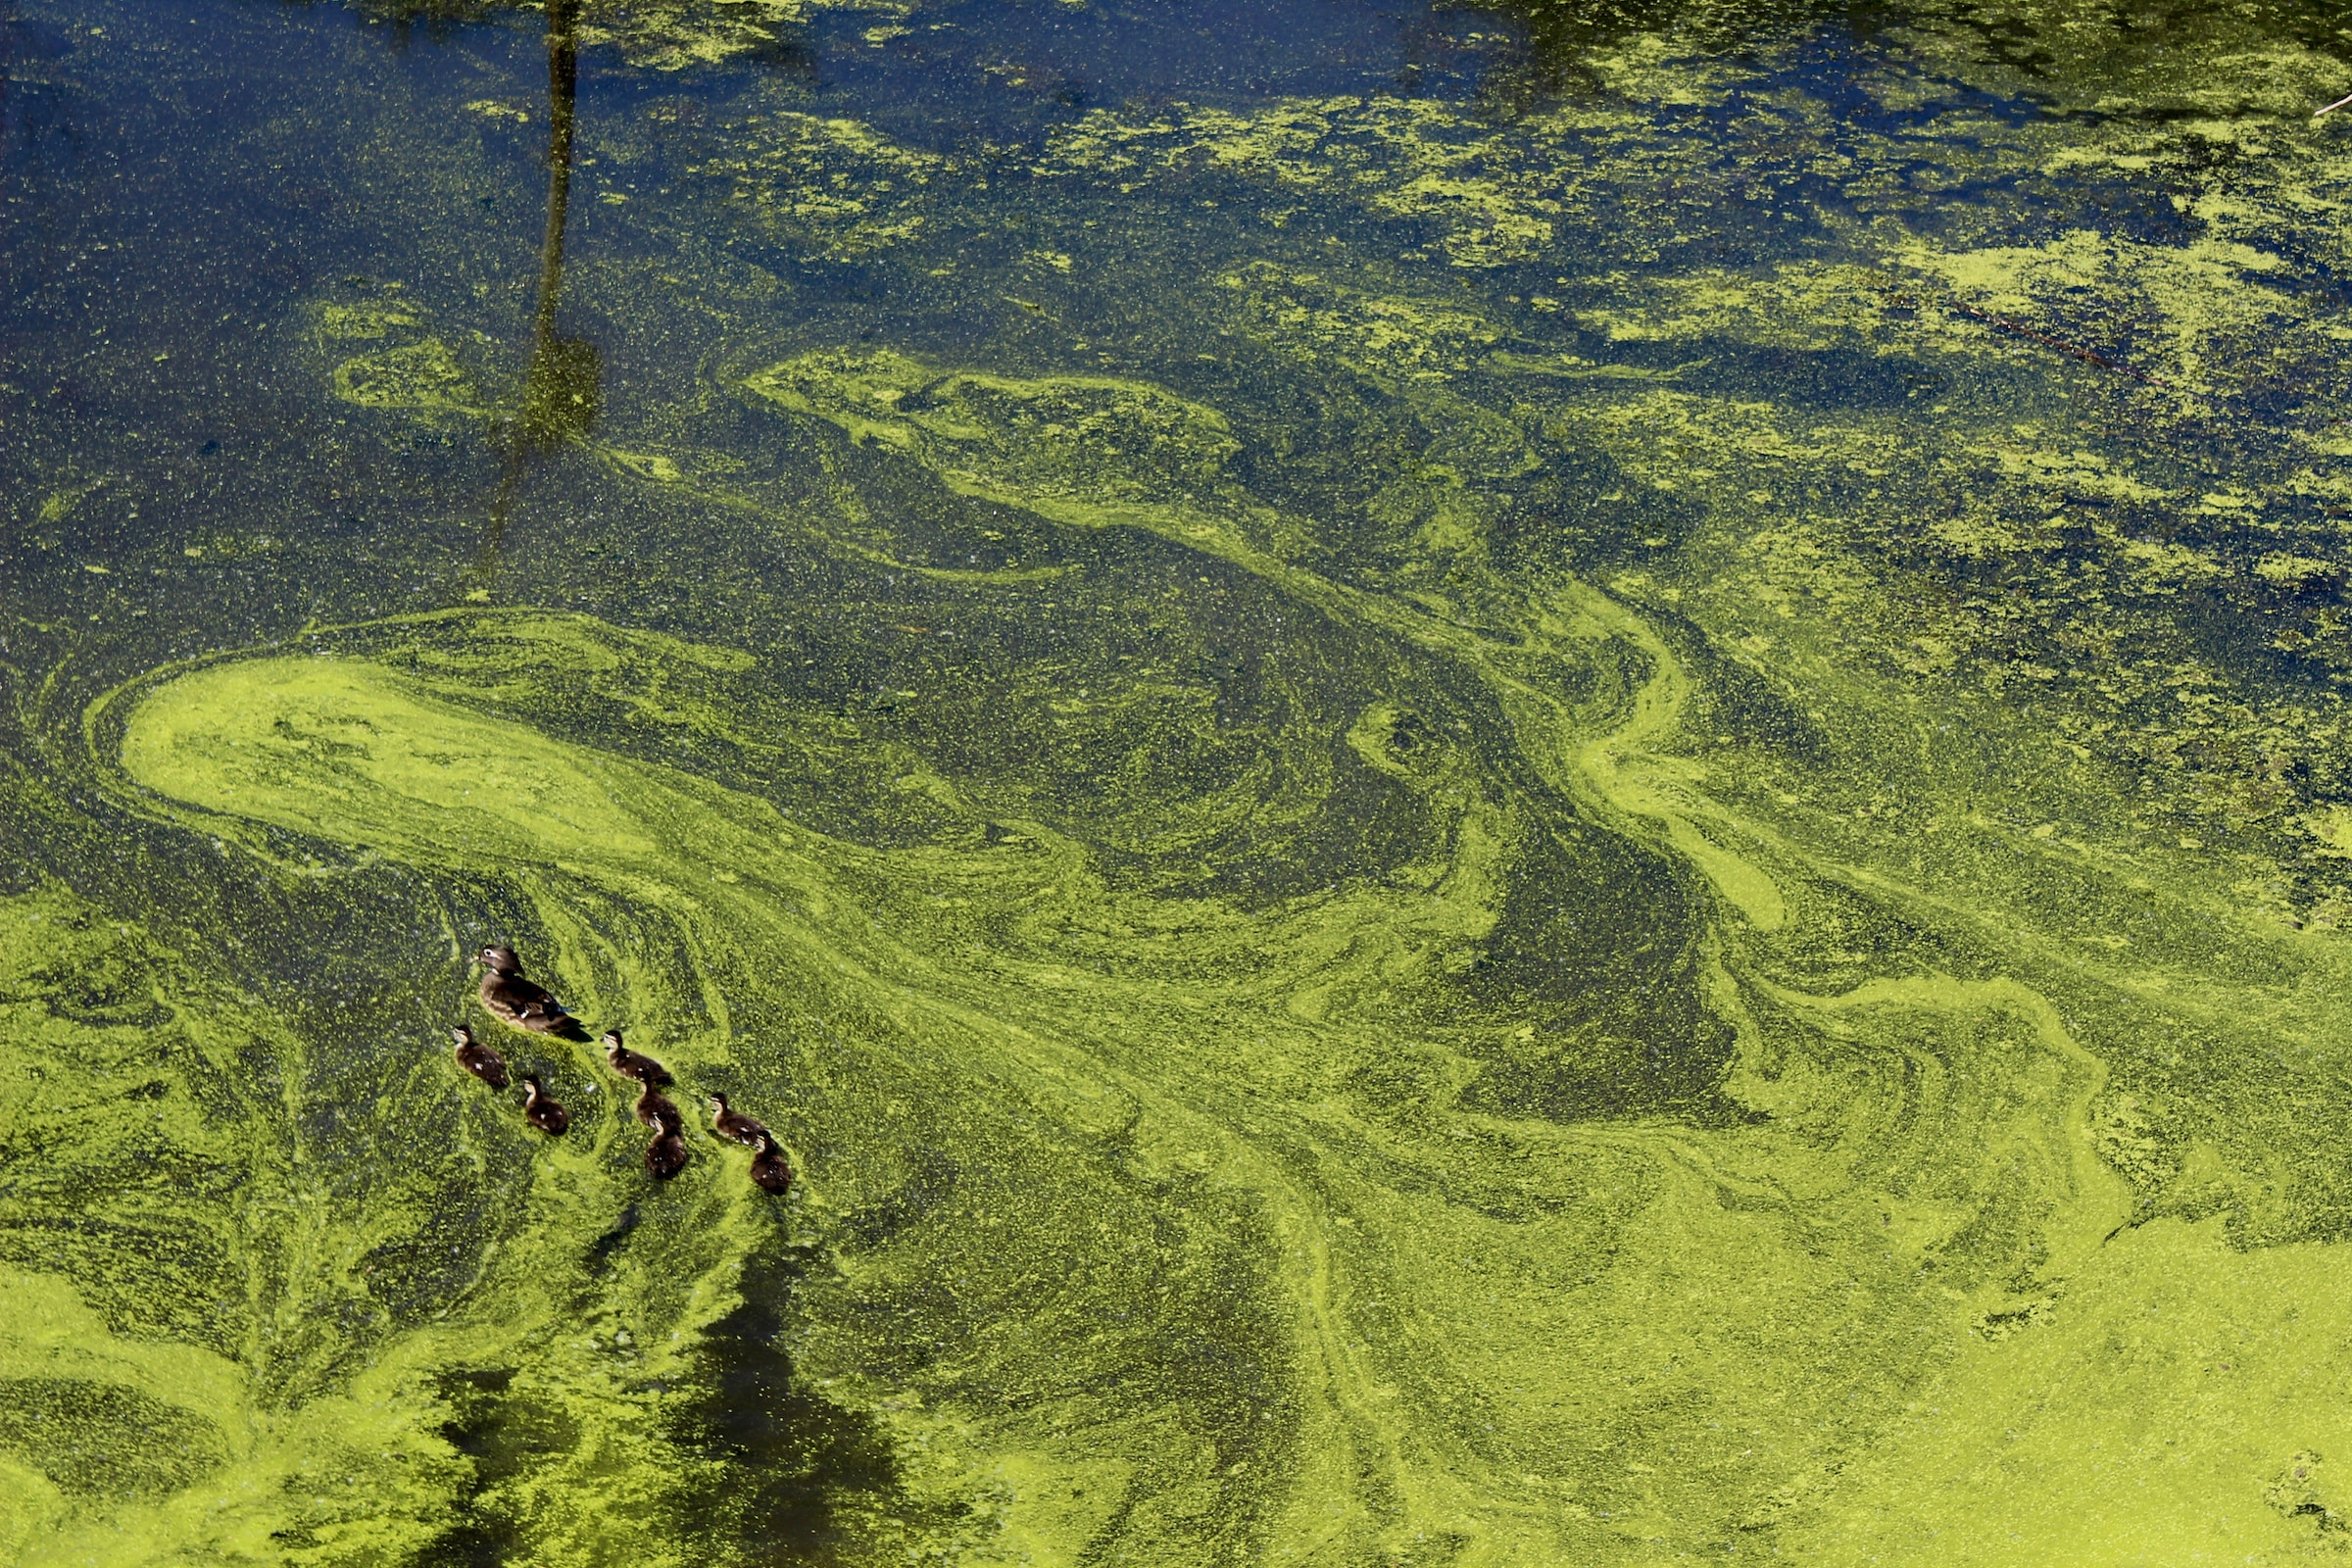
\includegraphics[width=1.1\textwidth]{figures/algae}
    \note<1>{WTP for \textbf{surface water} quality:
      \begin{itemize}
        \item Regulating and supporting services wrt. human health.
        \item Existence and bequest values.
        \item Outdoor recreation and option value.
        \item Aesthetic value.
      \end{itemize}
    }
    \note<2>{WTP for \textbf{groundwater} quality:
      \begin{itemize}
        \item Regulating and supporting services wrt. human health.
        \item The market for drinking water is imperfect, so we use stated preferences to capture the full value.
        \item Use value (with minimal treatment).
        \item Bequest values.
      \end{itemize}
    }
    \note<3>{Physical conditions can be worsened by stream straightening or intensive dredging and cutting of water weeds.
    }
    \note<4>{Nutrients, especially nitrate and phosphorus, are emitted from excessive use of fertilizers in agriculture and from point sources such as industry, cities, and sewage treatment plants.

    Eutrophication i.e. \textbf{(...)}
    }
\end{frame}